\section{Sistema de Comunicação}

\subsection{Visão Geral}

 Dois microcontroladores foram utilizados no sistema de comunicação: um para receber informações de temperatura (msp) e outro para fazer a comunicação com o módulo GPRS. O módulo GPRS possui uma antena GPS integrada, possibilitando enviar informações de localização para o raspberry PI. Além desses sinais, também é monitorado o fechamento da câmara, através do uso de um botão de fim de curso, e se ela está habilitada ou desabilitada, por meio do uso de uma chave. Todas essas informações são lidas pela raspberry PI e armazenadas em um banco de dados MySQL, sendo que a data e hora do report são recuperados pelo próprio sistema da raspberry. Um script escrito em python é responsável por ler informações da tabela do BD e enviar, sempre um registro por vez, os dados para o arduino. O arduino, por sua vez, é responsável por montar o arquivo JSON com as informações recebidas e enviar (POST) para a API, através do módulo GPRS, o qual permite uma conexão com a internet através da rede GSM. 

\begin{figure}[H]
	\centering
	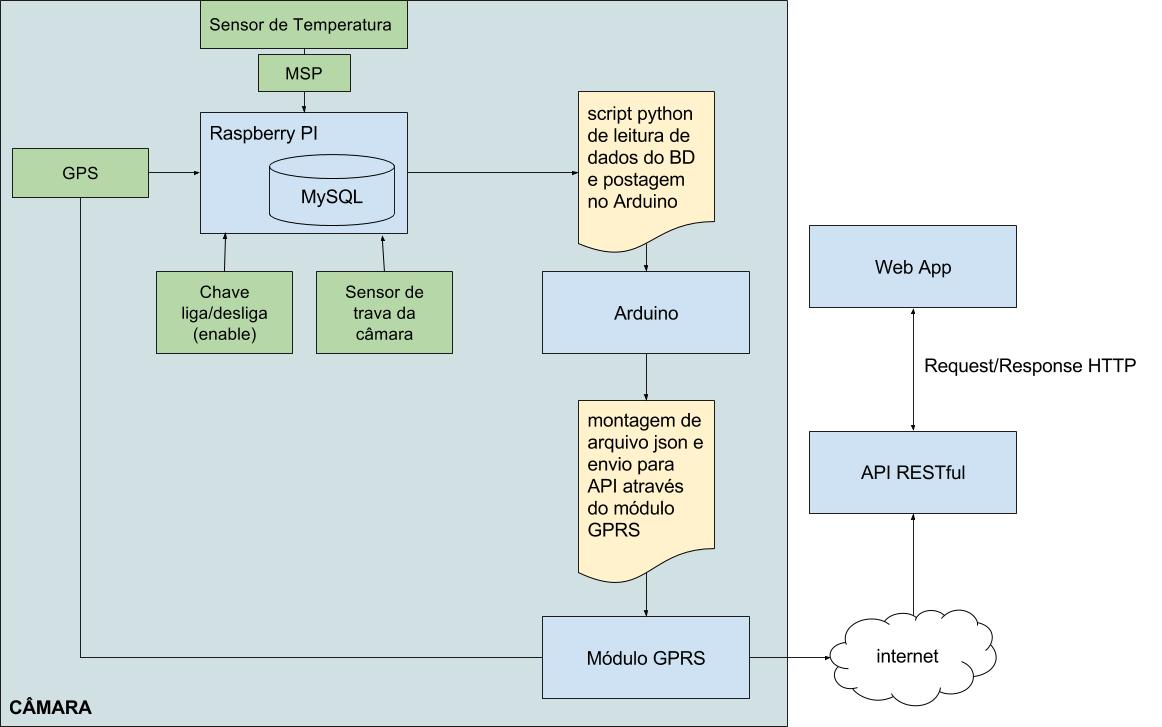
\includegraphics[width=16cm]{figuras/comunicacao_eletronica_software.jpg}
	\caption{Visão geral do sistema de comunicação}
\end{figure}

	
\subsection{Arquitetura de Software}
A arquitetura de software implementada consiste no modelo cliente-servidor. No server-side foi implementado uma API (webservice), em liguagem Python utilizando o framework Flask, que consiste na recepção e partilhamento dos dados advindos tanto do sistema web, quanto do sensoriamento da caixa transportadora, persistindo os dados e mantendo a segurança do sistema. O client-side consiste na aplicação web, com a qual o usuário interagir com o sistema, de acordo com seu nível de autorização. Foi implementado em linguagem Python + framework Django, seguindo o modelo de desenvolvimento MTV: Model - View - Template.

\begin{figure}[H]
	\centering
	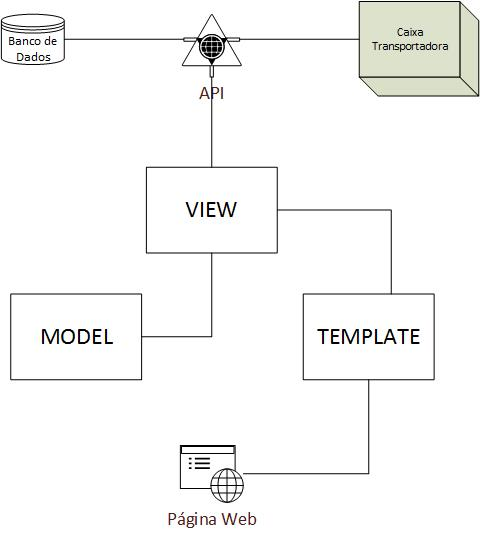
\includegraphics[width=12cm]{figuras/arquitetura_software.jpg}
	\caption{Arquitetura de Software}
\end{figure}
		
			
			\subsection{API}
			
			A API é o intermediário entre os sistemas e o banco de dados, uma forma de garantir que todos os dados sejam inseridos e recuperados através de um sistema em comum. Dessa forma podemos trabalhar com qualquer meio de visualização de dados e métodos de inserção, que se torna imprescindível para o funcionamento de um sistema onde temos uma interface WEB e um equipamento eletrônico que irá inserir dados no banco de dados.
			
			A caixa transportadora acessará a API para fornecer as leituras dos sensores de localização, temperatura, fechamento e os dados do transporte. A API tratará de armazenar esses dados no banco através dos endpoints configurados. A partir daí o sistema WEB pode recuperar esses dados com chamadas nos endpoints da API. 
			
			Portanto a caixa transportadora servirá somente como interface de inserção de dados enquanto o WEB app funcionará como inserção e recuperação. A API foi documentada na plataforma POSTMAN que automatiza e testa os endpoints configurados\footnote{Link para a documentação: \href{https://documenter.getpostman.com/view/579285/transorg/6tXcSQ7}{https://documenter.getpostman.com/view/579285/transorg/6tXcSQ7} Link para o repositório: \href{https://github.com/TransportadoraOrgaos/restfull-api}{https://github.com/TransportadoraOrgaos/restfull-api}}. 
			
			A seguir a tela da ferramenta com a api configurada:
			
			\begin{figure}[H]
				\centering
				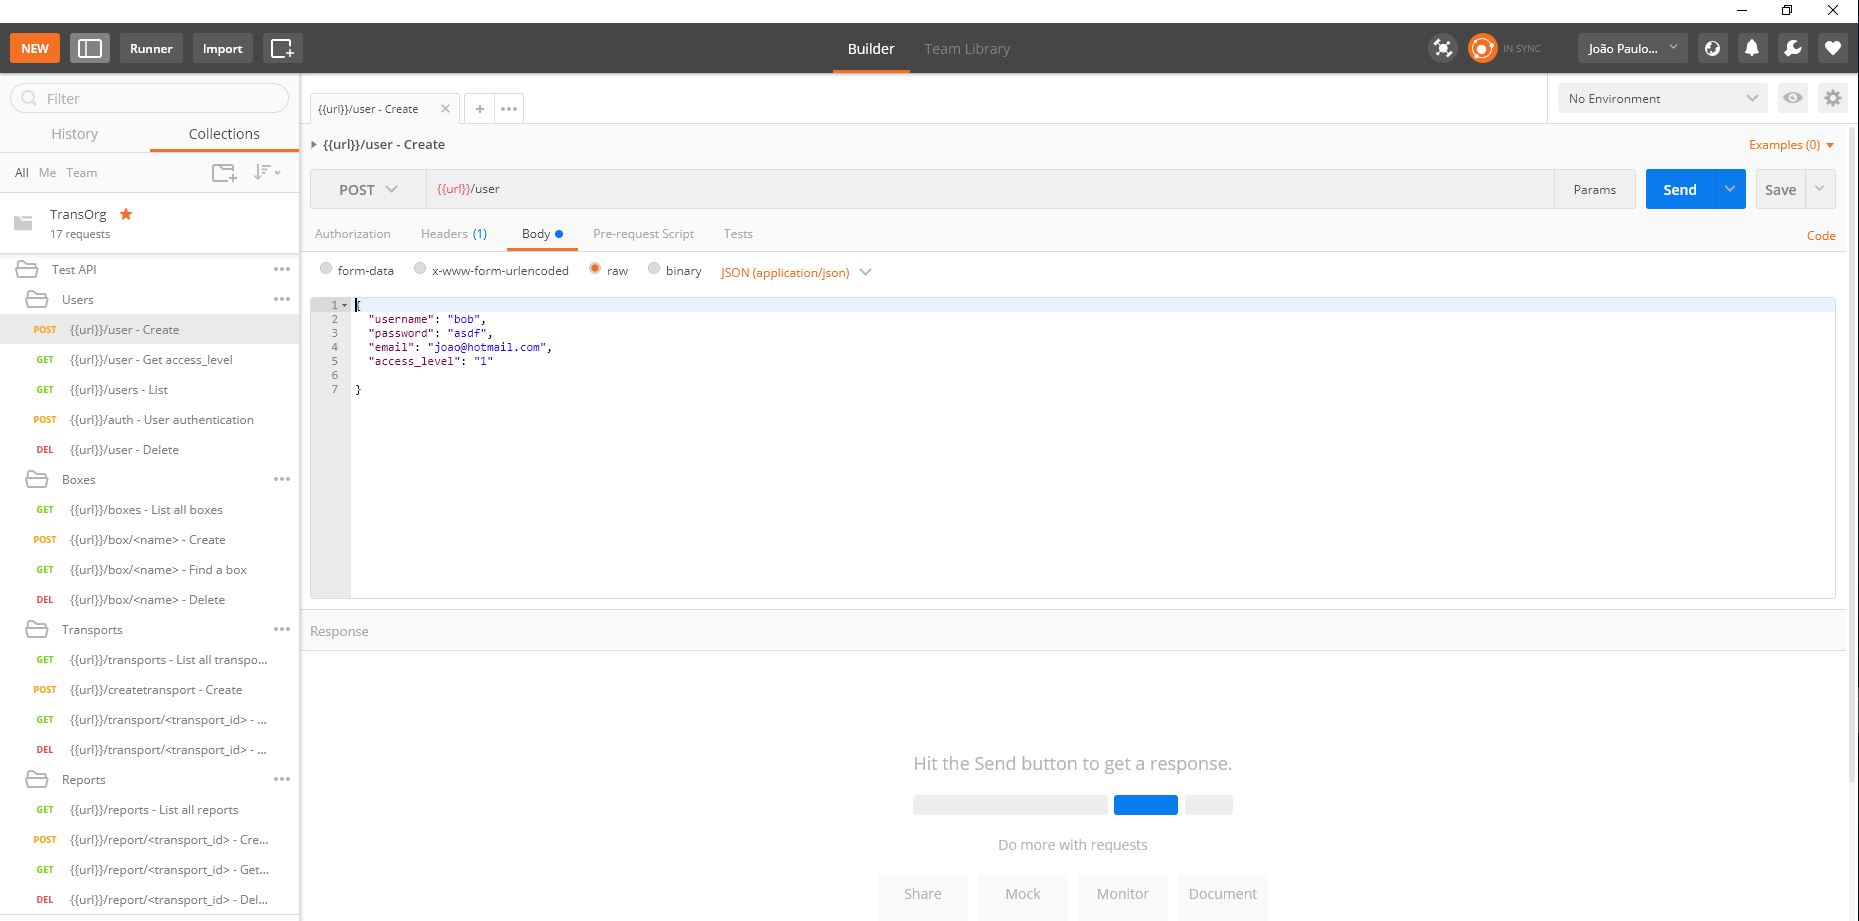
\includegraphics[width=16cm]{figuras/api_software.JPG}
				\caption{API do Sistema}
			\end{figure}
	
			
			
			
			
			
\section{Sistema WEB}

\subsection{Diagrama de classes}

\begin{figure}[H]
	\centering
	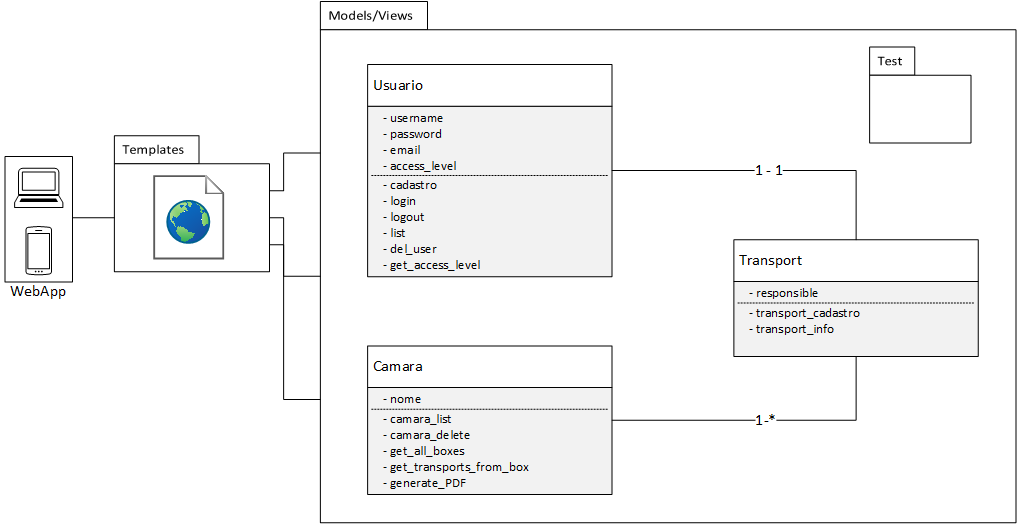
\includegraphics[width=16cm]{figuras/diagrama_classe.png}
	\caption{Diagrama de classes}
\end{figure}


\subsection{Cadastro de Usuários}
	Foi implementado um sistema de cadastro de usuários, aos quais estes serão classificados e cadastrados em três diferentes tipos de acordo com seu nível de autorização.

\begin{itemize}
\item Administrador: Terá controle total sobre a aplicação; somente usuário administrador terá acesso aos cadastros de usuários e novas câmaras de transporte;
\item Transportador:  Terá autorização para iniciar um novo transporte e visualizar o andamento do mesmo;
\item Usuário: Poderá apenas visualizar as informações de um transporte em andamento.
\end{itemize}

	Para o cadastro serão necessários informar os dados de nome de usuário, email, senha e nível de acesso. A seguir a tela de cadastro:

\begin{figure}[H]
\centering
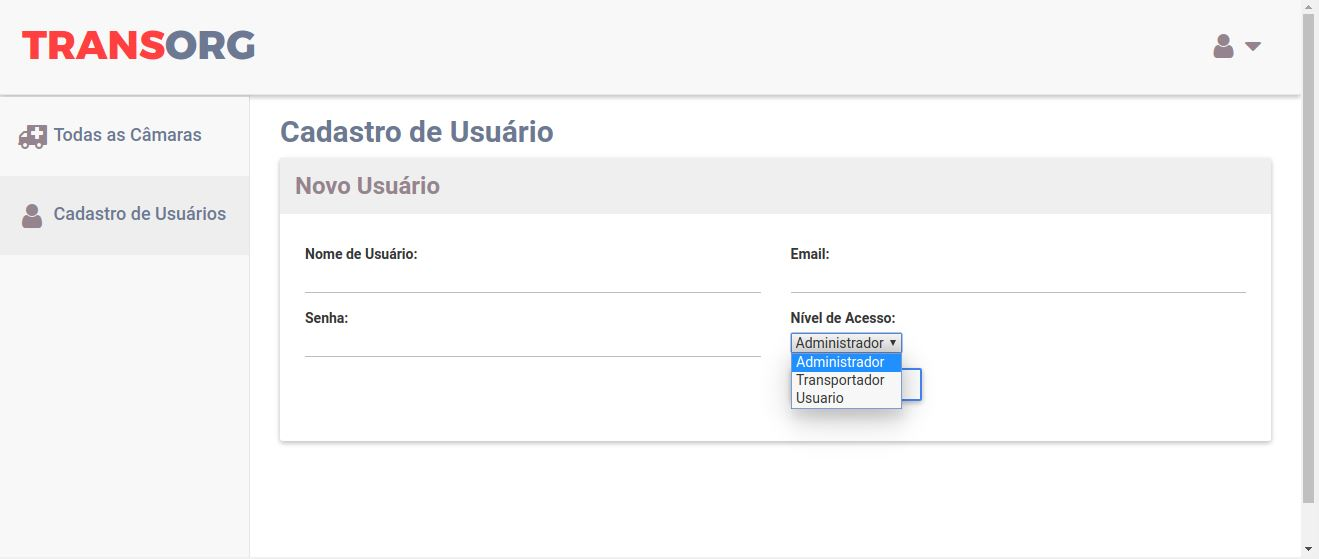
\includegraphics[width=16cm]{figuras/cadastro_software.JPG}
\caption{Arquitetura de Software}
\end{figure}

\subsection{Listar e Apagar Usuários}
	O sistema irá dispor de uma página específica para listar todos os usuários cadastrados juntamente com a opção de deletar os mesmos. A seguir a tela de listagem de usuários:

\begin{figure}[H]
\centering
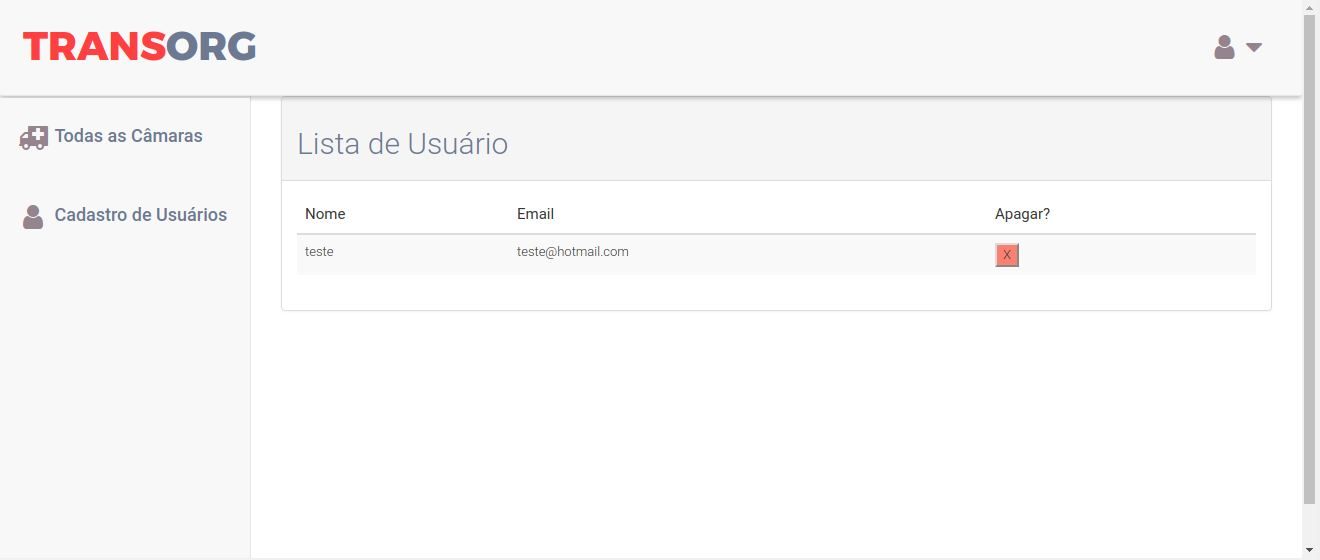
\includegraphics[width=16cm]{figuras/listaUsuarios_software.JPG}
\caption{Listar usuários}
\end{figure}

\subsection{Sistema de Login}
	O sistema de autenticação se dará por meio do envio dos dados das credenciais à API, composto por nome de usuário e senha, e caso estas informações estejam corretas a API retorna um token de acesso ao qual é guardado em uma sessão, onde para acesso às páginas, o sistema sempre verificará se consta na sessão o token correto, caso contrário retornará à página de login. 
	
	A seguir a tela de Login:

\begin{figure}[H]
\centering
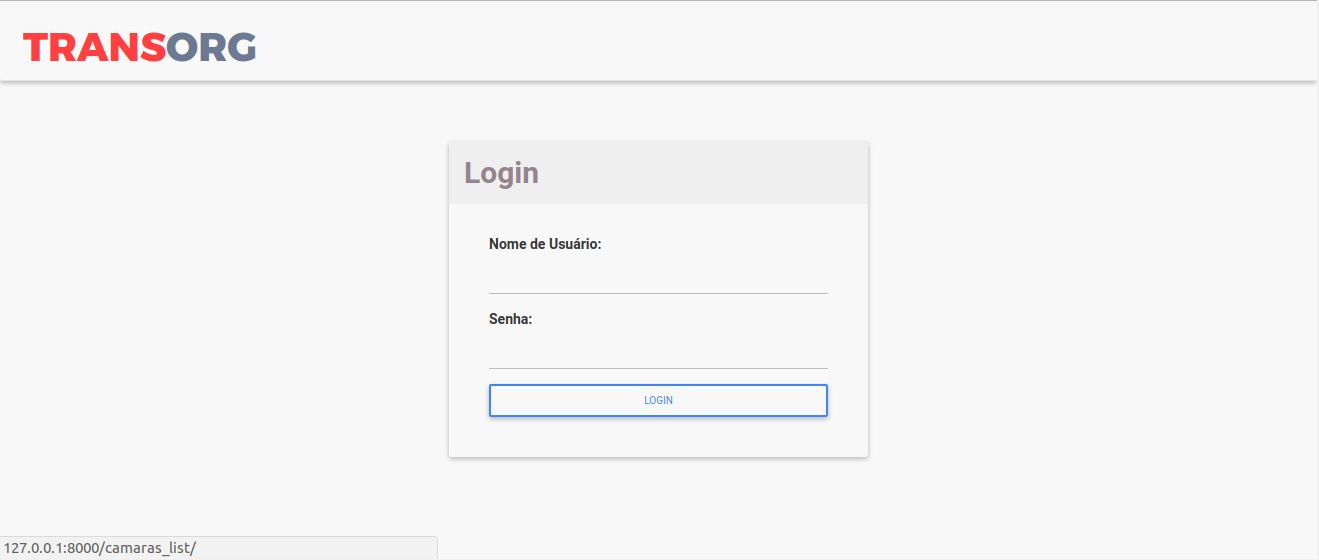
\includegraphics[width=16cm]{figuras/login_software.JPG}
\caption{Login no WebApp}
\end{figure}

\subsection{Cadastro de Câmaras}
	O sistema dispõe de um cadastro de novas câmaras, onde é solicitado o nome da mesma para seu cadastro. Internamente é criada junto ao webservice com seu id relacionado. A partir de sua criação, esta câmara já fica disponível para transporte no sistema.
	
	A seguir a tela de cadastro de câmaras:

\begin{figure}[H]
\centering
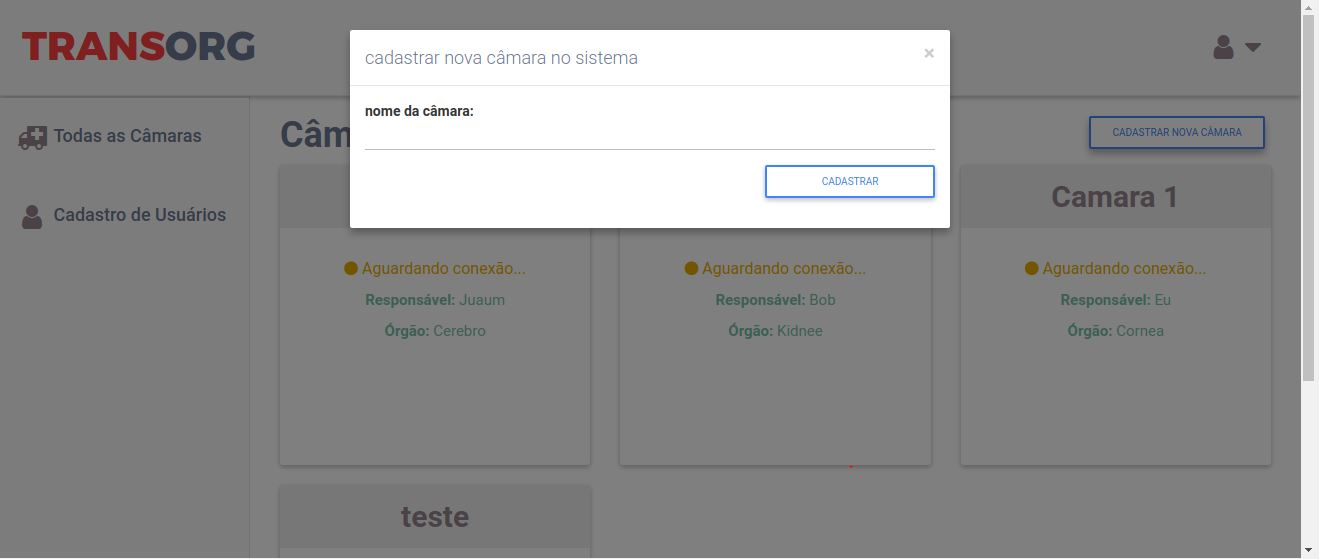
\includegraphics[width=16cm]{figuras/cadastroCamaras_software.JPG}
\caption{Cadastro de Câmaras}
\end{figure}

\subsection{Visualizar Todas as Câmaras}
	A tela principal do sistema se dará pela visualização das câmaras disponíveis e em uso, a partir dela será possível iniciar novas solicitações de transporte. Câmaras disponíveis e fora de uso também há a opção de deleção.
	
	A seguir tela de visualização de câmaras:

\begin{figure}[H]
\centering
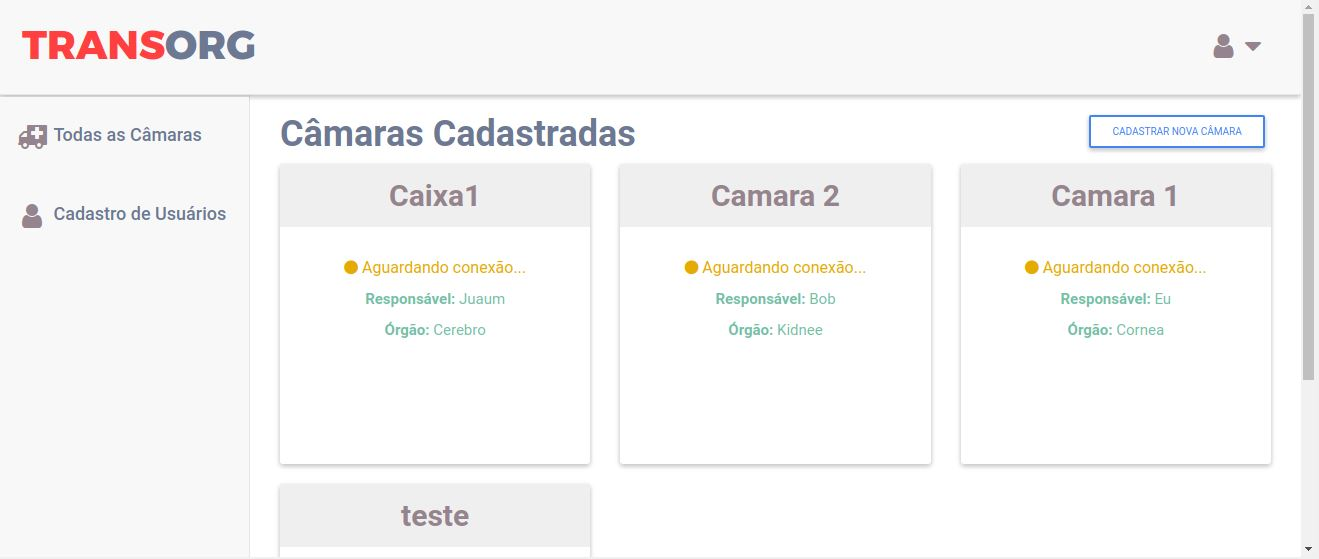
\includegraphics[width=16cm]{figuras/listaCamaras_software.JPG}
\caption{Listar Câmaras}
\end{figure}

\subsection{Iniciar Novo Transporte}
	A partir da seleção de uma câmara disponível o usuário é redirecionado à página de início de um novo transporte onde é solicitado informar o responsável pelo transporte e o órgão ao qual será transportado.
	
	A seguir a tela de início de um novo transporte:

\begin{figure}[H]
\centering
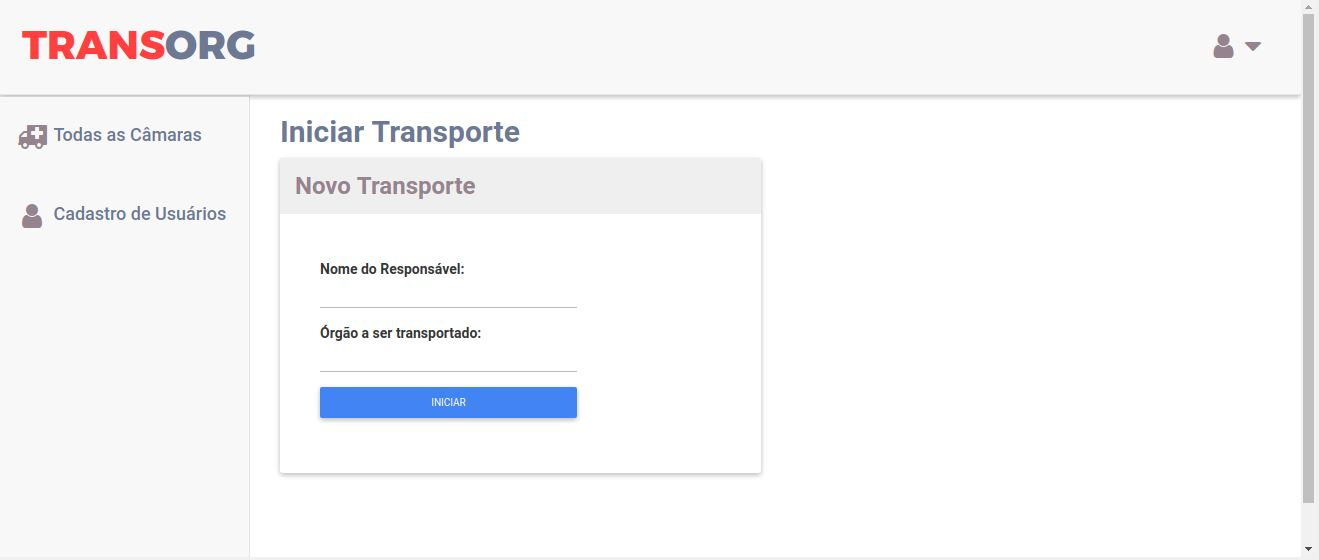
\includegraphics[width=16cm]{figuras/iniciarTransporte_software.JPG}
\caption{Iniciar Transporte}
\end{figure}

\subsection{Visualizar Transporte em Andamento}
	A principal funcionalidade do sistema, onde se é possível visualizar todas as informações de um transporte em andamento. As informações apresentadas são: gráfico de temperatura, temperatura atual, localização atual, responsável pelo transporte, órgão transportado, status da trava de segurança e data e hora destes dados.

	A seguir tela de visualização de andamento de um transporte ativo:

\begin{figure}[H]
\centering
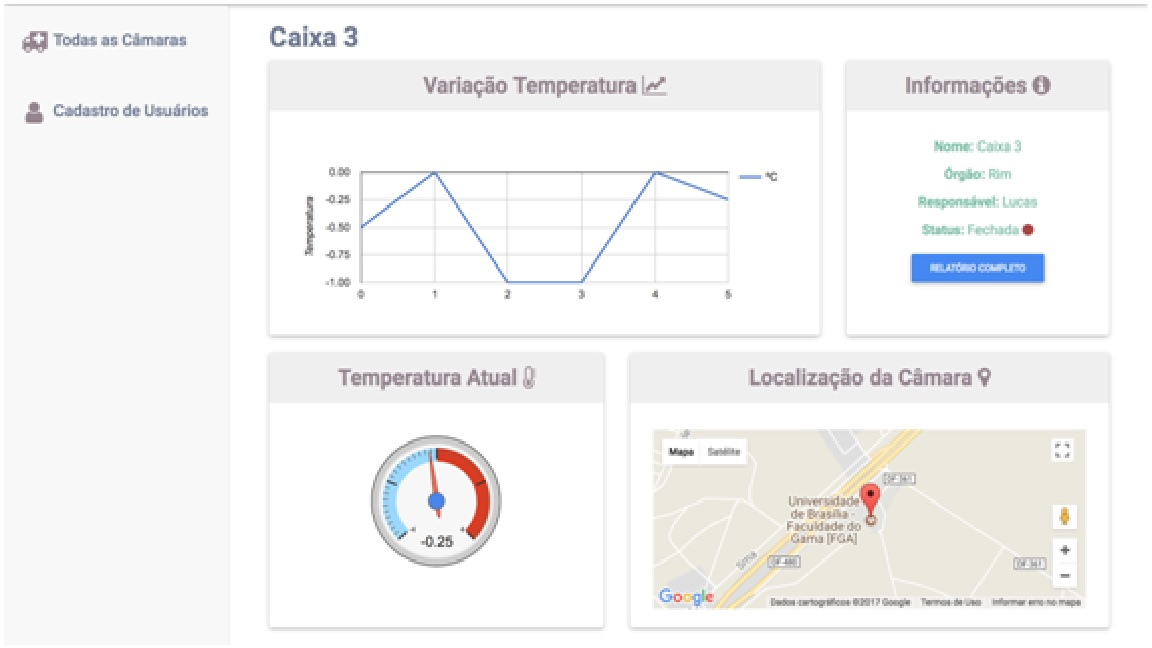
\includegraphics[width=16cm]{figuras/camara_software.jpg}
\caption{Câmara de transporte}
\end{figure}

\subsection{Relatório}
	O sistema dispõe de uma funcionalidade de relatório, ao qual o usuário irá visualizar as informações dos transportes realizados, com opção de exportação em PDF.
	A seguir tela de relatório:
\begin{figure}[H]
\centering
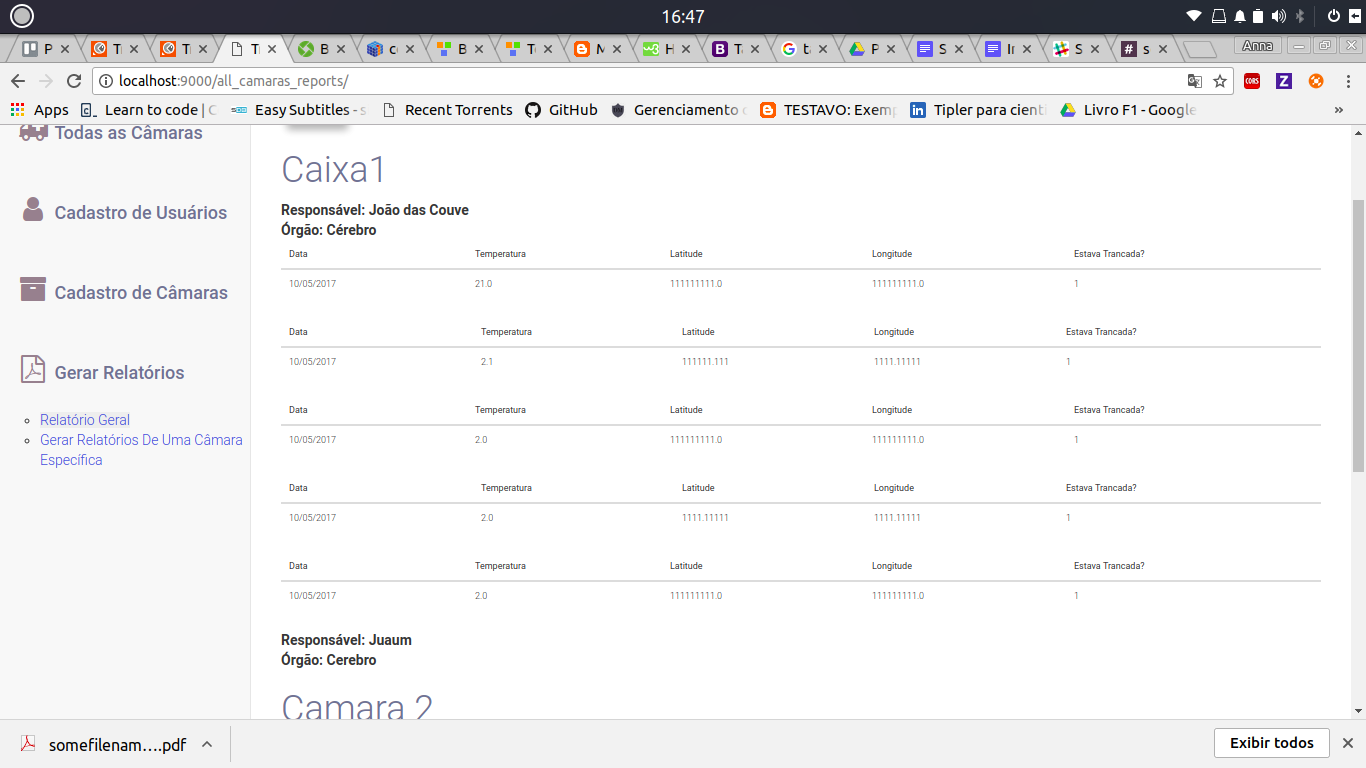
\includegraphics[width=16cm]{figuras/relatorio_software.png}
\caption{Relatórios do sistema}
\end{figure}

\subsubsection{Integração contínua}

Para o desenvolvimento da aplicação web, foi estabelecido um fluxo de trabalho conforme ilustrado pela figura \ref{integra_continua}. Para cada desenvolvedor, foi criado uma branch para codificar, rodar os testes automatizados, realizar o commit e dar o push. A cada novo push, era criado uma nova build no travis da branch correspondente. Quando a branch atingia um nível aceitável, o desenvolvedor realizava o merge com a branch development. Uma nova bateria de testes era rodada nessa branch. Ao realizar o push, além de ser criada uma nova build no Travis, era feito o deploy em uma aplicação 'transorg-dev' no Heroku. Quando a branch development atingia um nível estável, era feito um pull request na master. Todos os desenvolvedores deveriam avaliar o pull request antes do merge ser realizado. Uma vez realizado o merge e o push da master, além de ser criado uma nova build no Travis, era feito um deploy na aplicação 'transorg' no Heroku \footnote{Link para o repositório: \href{https://github.com/TransportadoraOrgaos/pi2-transport_orgaos}{https://github.com/TransportadoraOrgaos/pi2-transport\_orgaos}.\newline Link para o Travis: \href{https://travis-ci.org/TransportadoraOrgaos/pi2-transport\_orgaos/branches}{https://travis-ci.org/TransportadoraOrgaos/pi2-transport\_orgaos/branches}.\newline Link para aplicação no Heroku: \href{https://transorg.herokuapp.com}{https://transorg.herokuapp.com}}.

\begin{figure}[H]
	\centering
	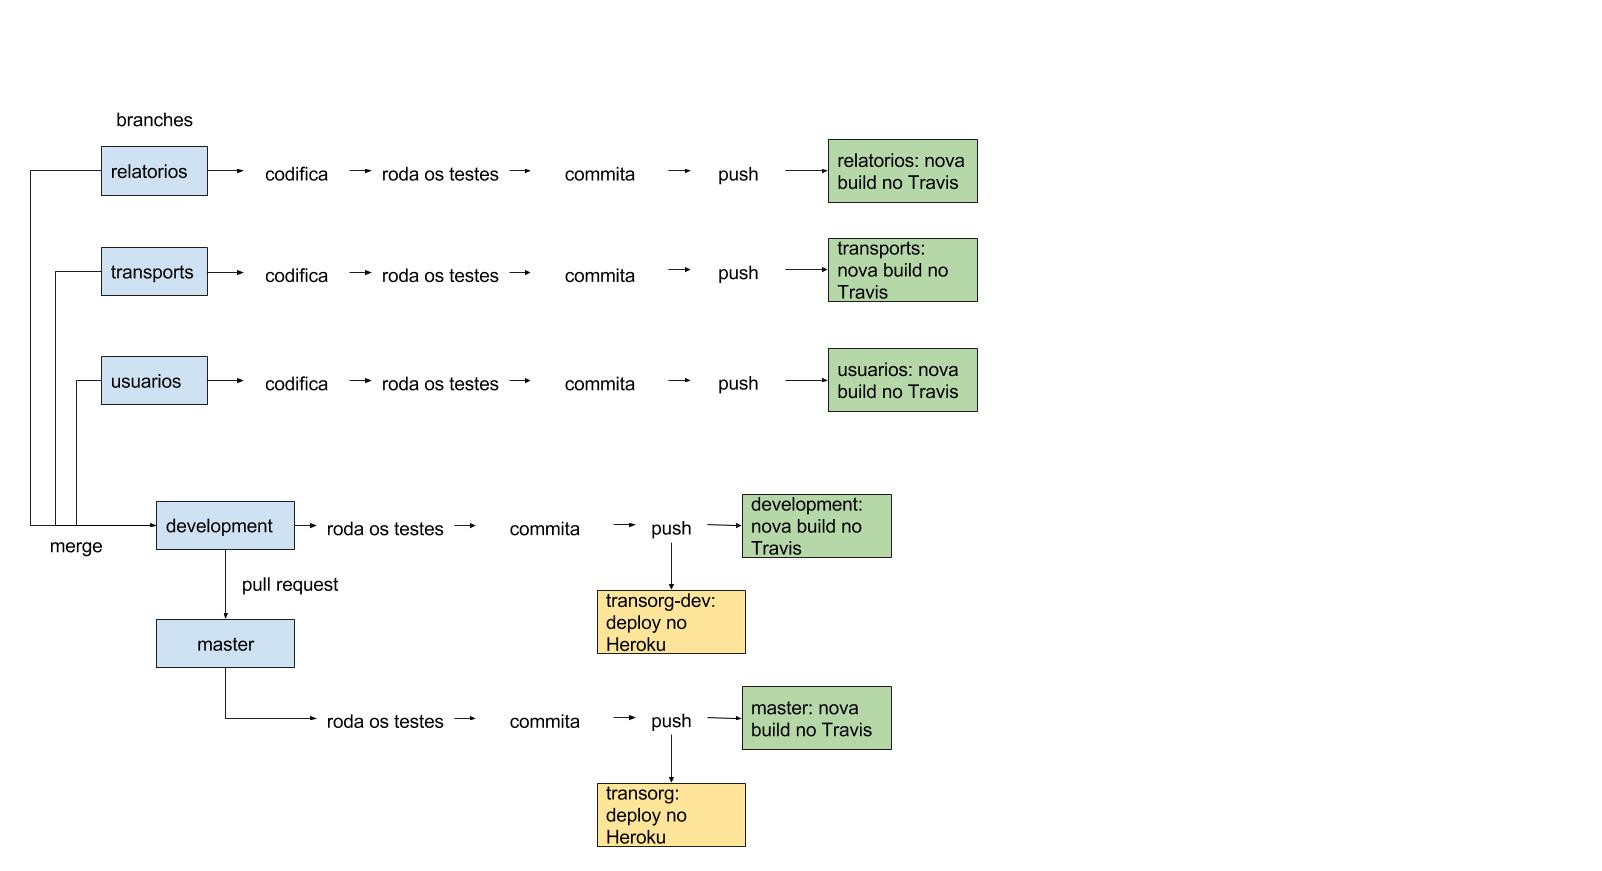
\includegraphics[width=24cm]{figuras/integracao_continua.jpg}
	\caption{Integração Contínua} \label{integra_continua}
\end{figure}

A figura \ref{travis} mostra as builds realidas pelo Travis:

\begin{figure}[H]
	\centering
	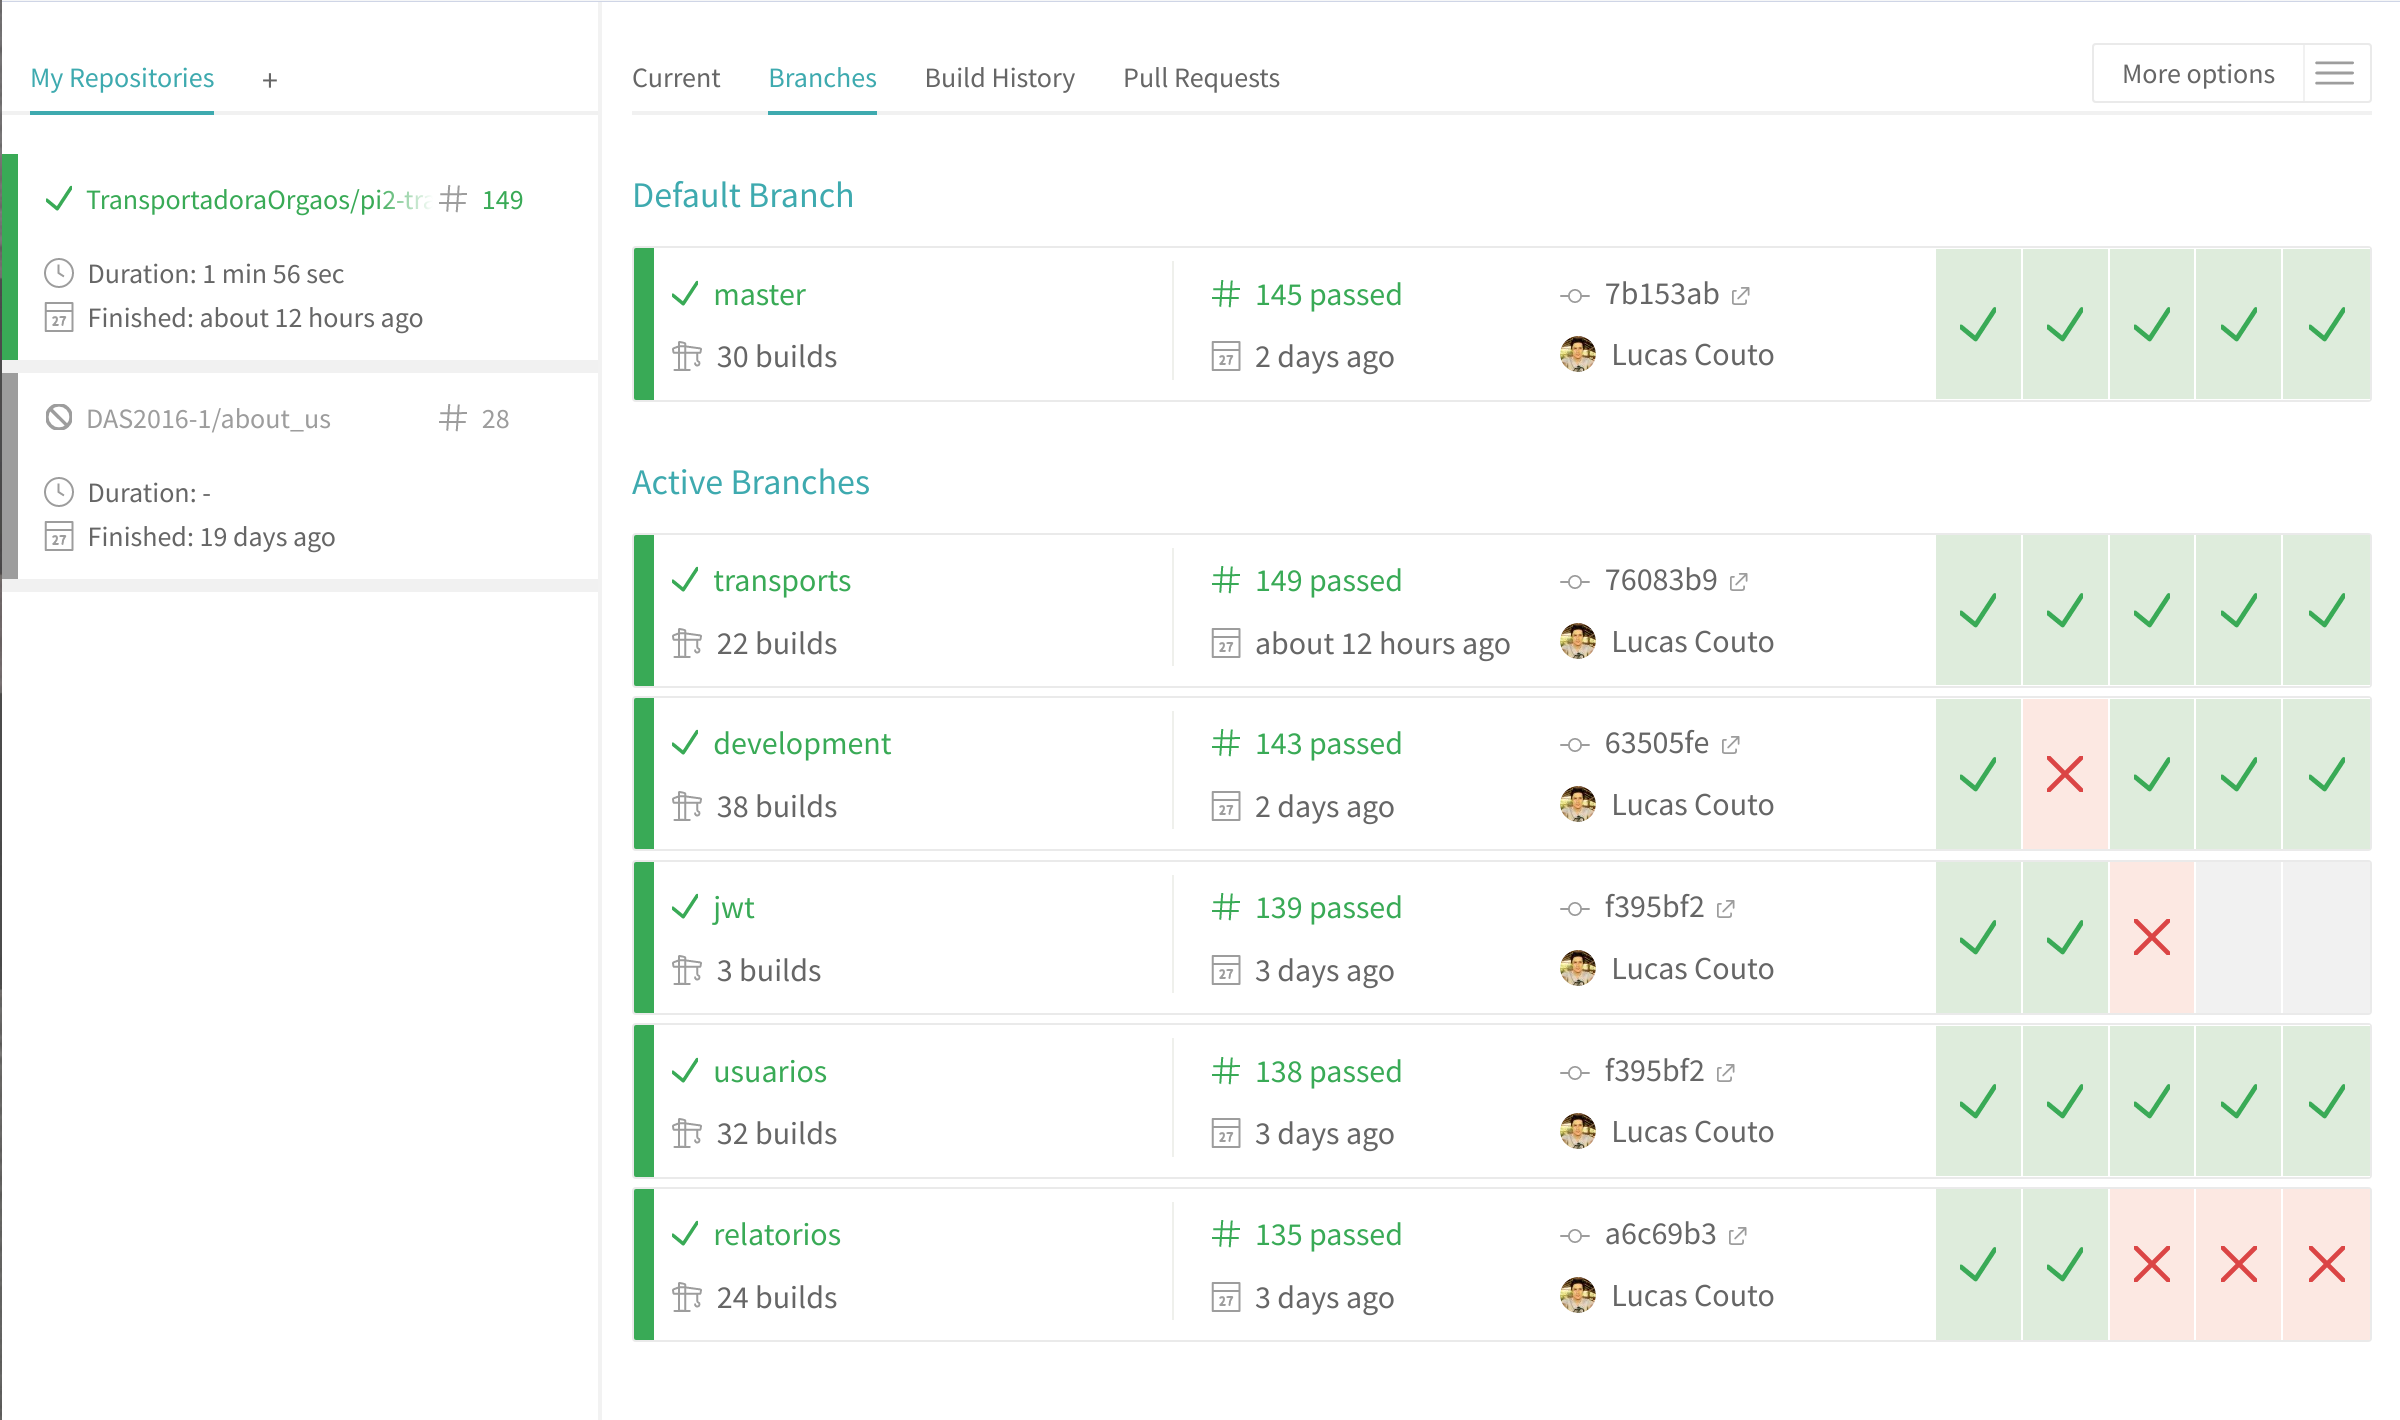
\includegraphics[width=16cm]{figuras/travis.png}
	\caption{Builds no Travis} \label{travis}
\end{figure}

A figura \ref{cobertura_codigo} mostra a cobertura do código dos testes realizados:

\begin{figure}[H]
	\centering
	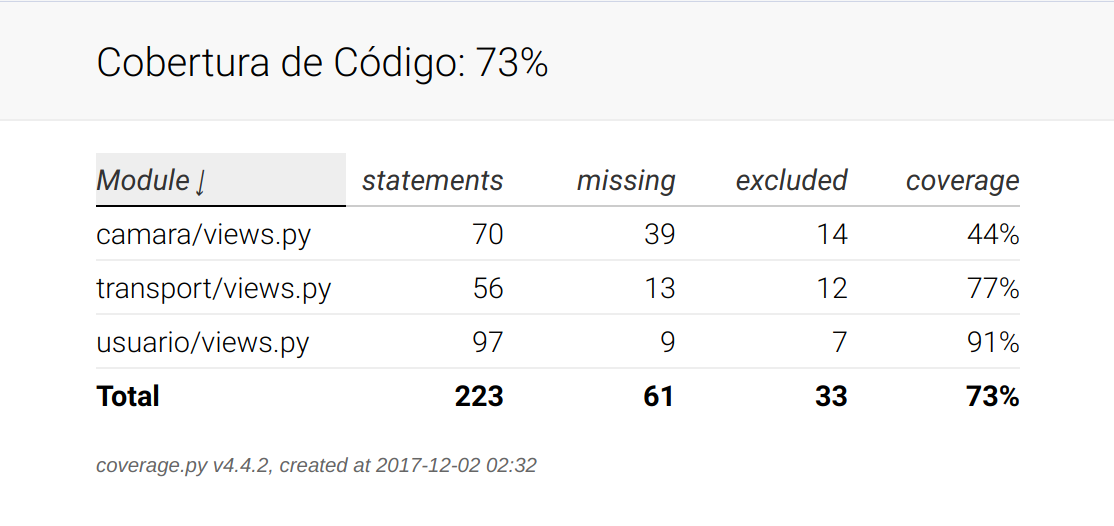
\includegraphics[width=14cm]{figuras/cobertura_codigo.png}
	\caption{Cobertura de Código} \label{cobertura_codigo}
\end{figure}




